%   ------------------------------------------------------------------------
\FloatBarrier
\section{Animated Drawnings}
\label{s.sketchApendice}

\begin{figure}[htbp]
    \centering
    \caption{Tela Inicial do Animated Drawnings}
    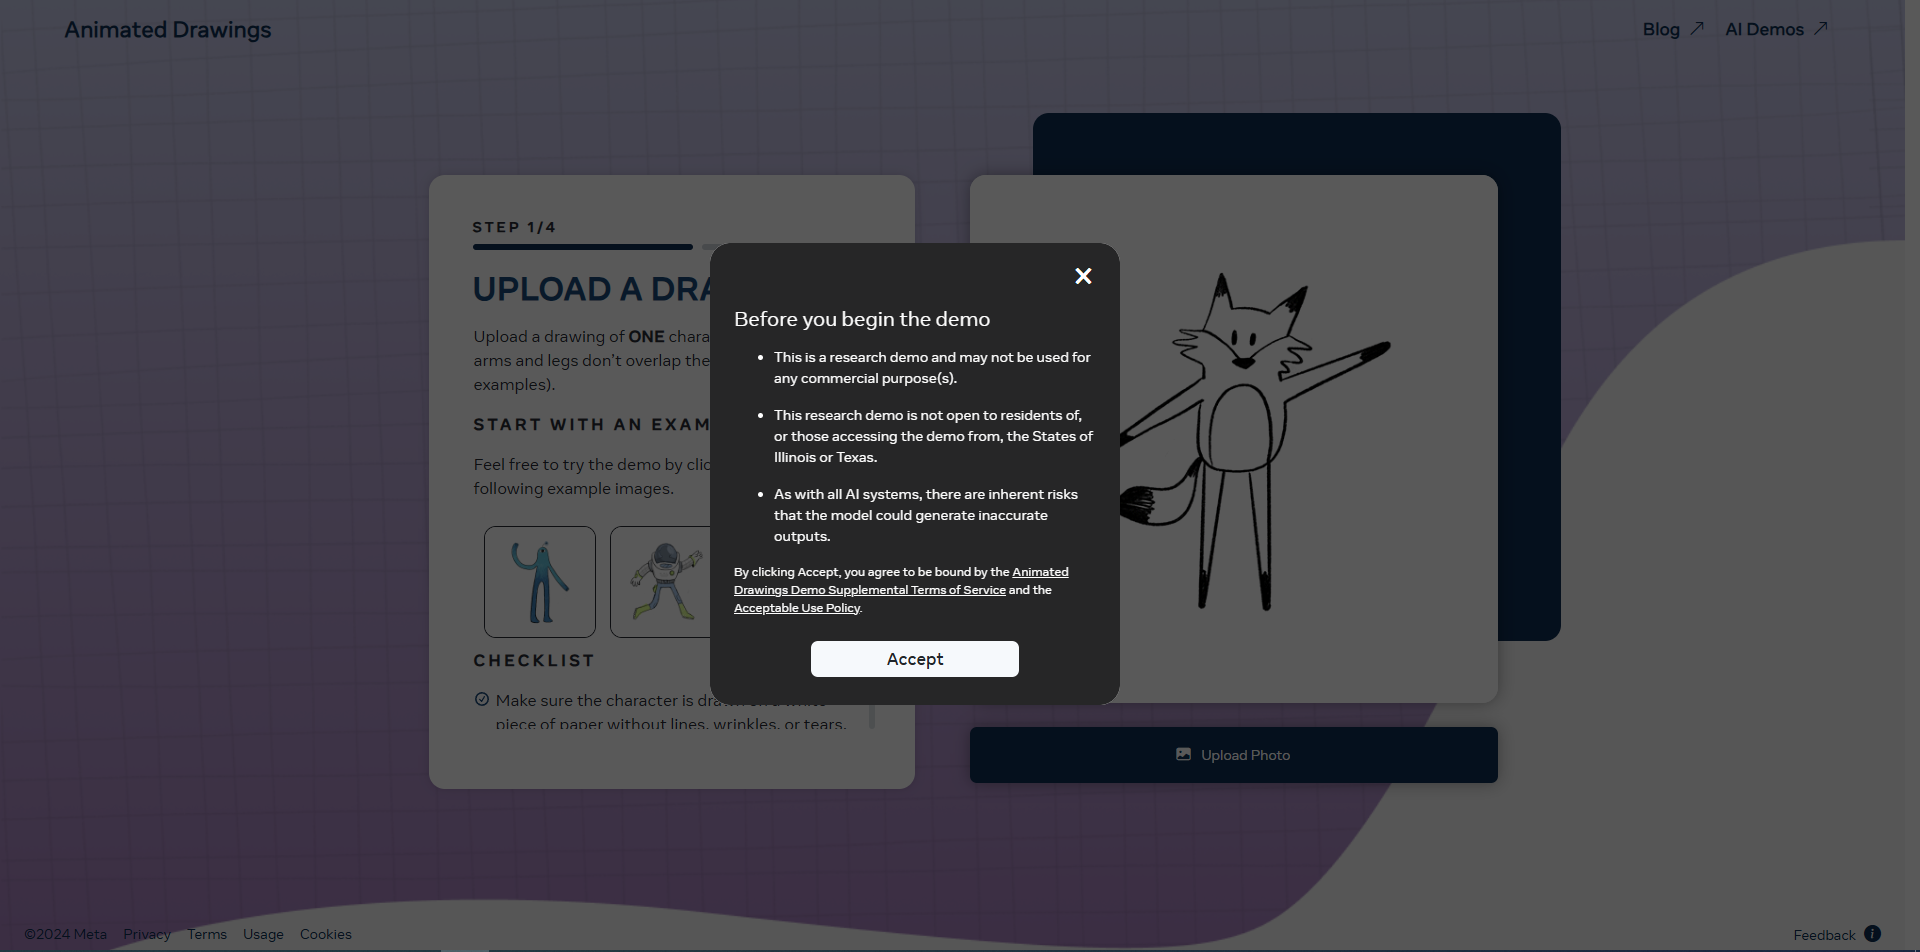
\includegraphics[width=1\linewidth]{figs/sketchLab/telaInicial.PNG}
    \label{fig:sketchInicial}
\end{figure}

\begin{figure}[htbp]
    \centering
    \caption{Requisitos do desenho a ser enviado}
    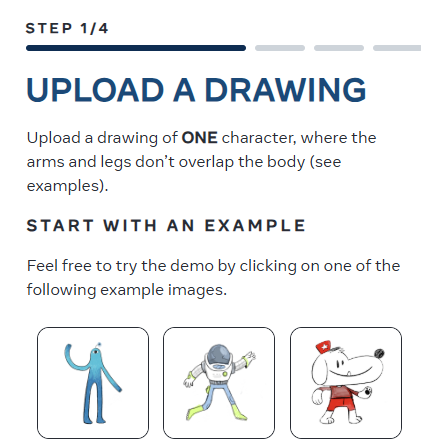
\includegraphics[width=0.5\linewidth]{figs/sketchLab/semSobreposicao.PNG}
    \label{fig:sketchSobreposicao}
\end{figure}

\begin{figure}[htbp]
    \centering
    \caption{\small Processo da utilização 1 do Animated Drawnings}
    \label{fig:sketch1}
    \begin{subfigure}{0.45\linewidth}
        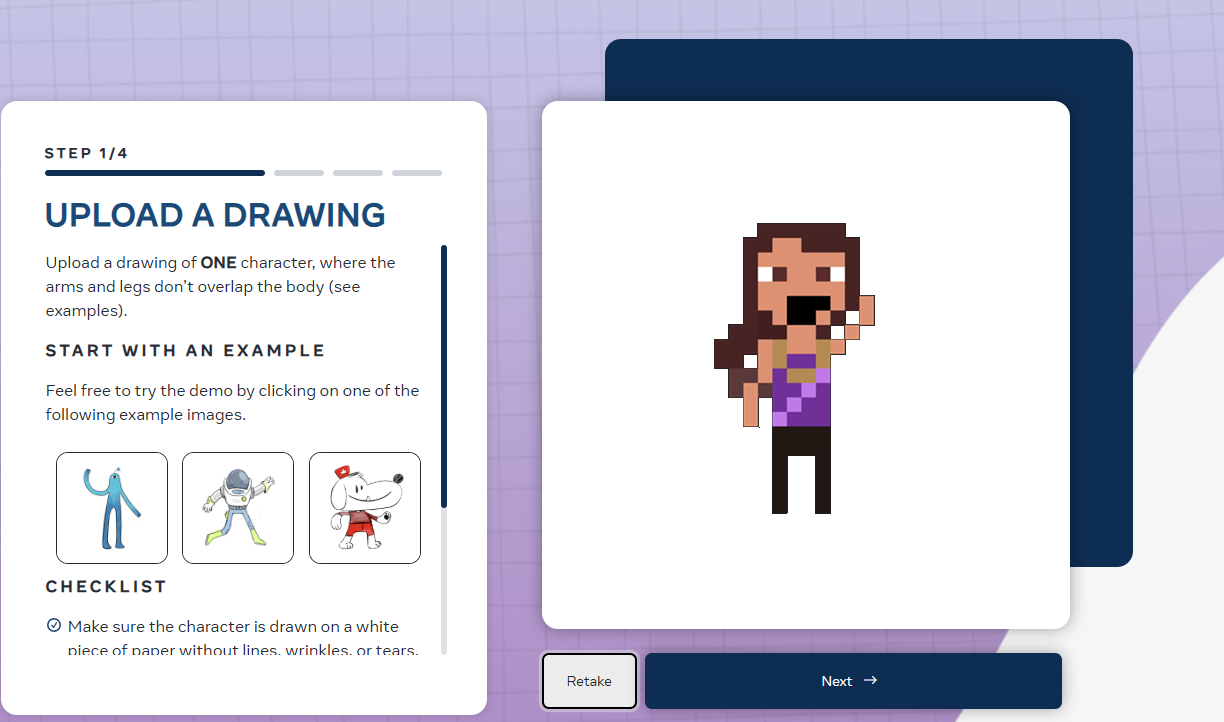
\includegraphics[width=1\linewidth]{figs/sketchLab/tela1.PNG}
        \caption{\small Desenho enviado.}
        \label{fig:sketch1a}
    \end{subfigure}
    \begin{subfigure}{0.45\linewidth}
        \centering
        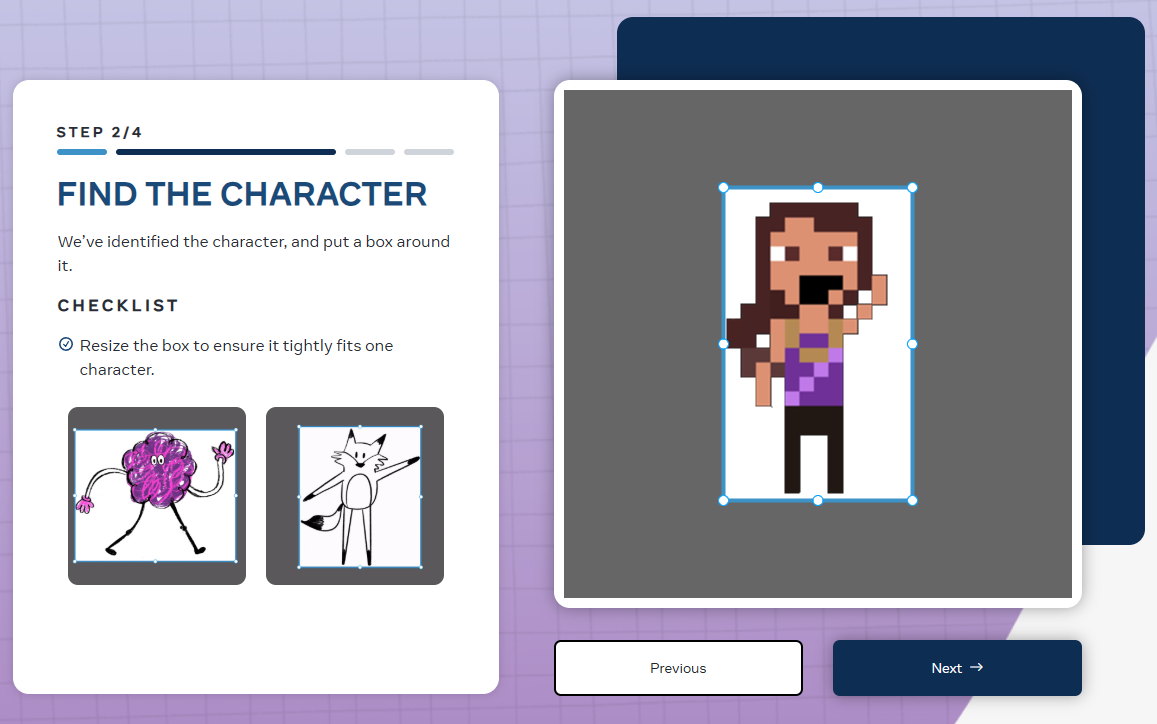
\includegraphics[width=1\linewidth]{figs/sketchLab/tela2.PNG}
        \caption{\small Encontrar personagem.}
        \label{fig:sketch1b}
    \end{subfigure}
    \begin{subfigure}{0.45\linewidth}
        \centering
        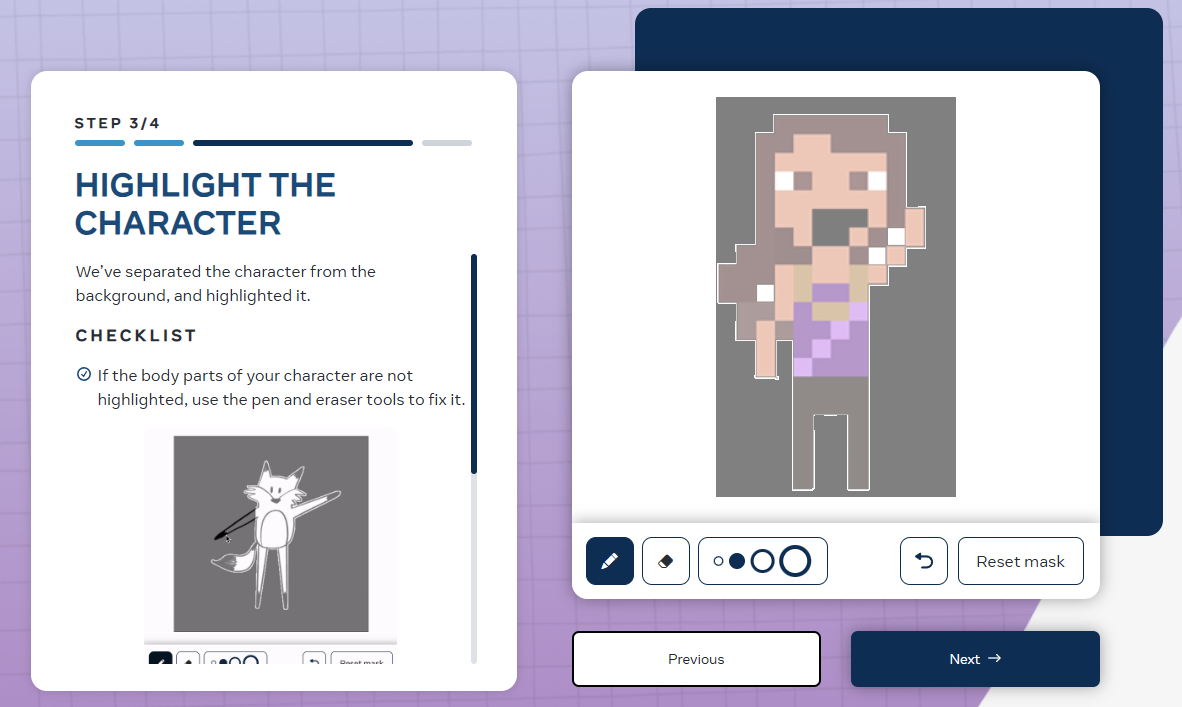
\includegraphics[width=1\linewidth]{figs/sketchLab/tela3.PNG}
        \caption{\small Destacar personagem automático.}
        \label{fig:sketch1c}
    \end{subfigure}
    \begin{subfigure}{0.45\linewidth}
        \centering
        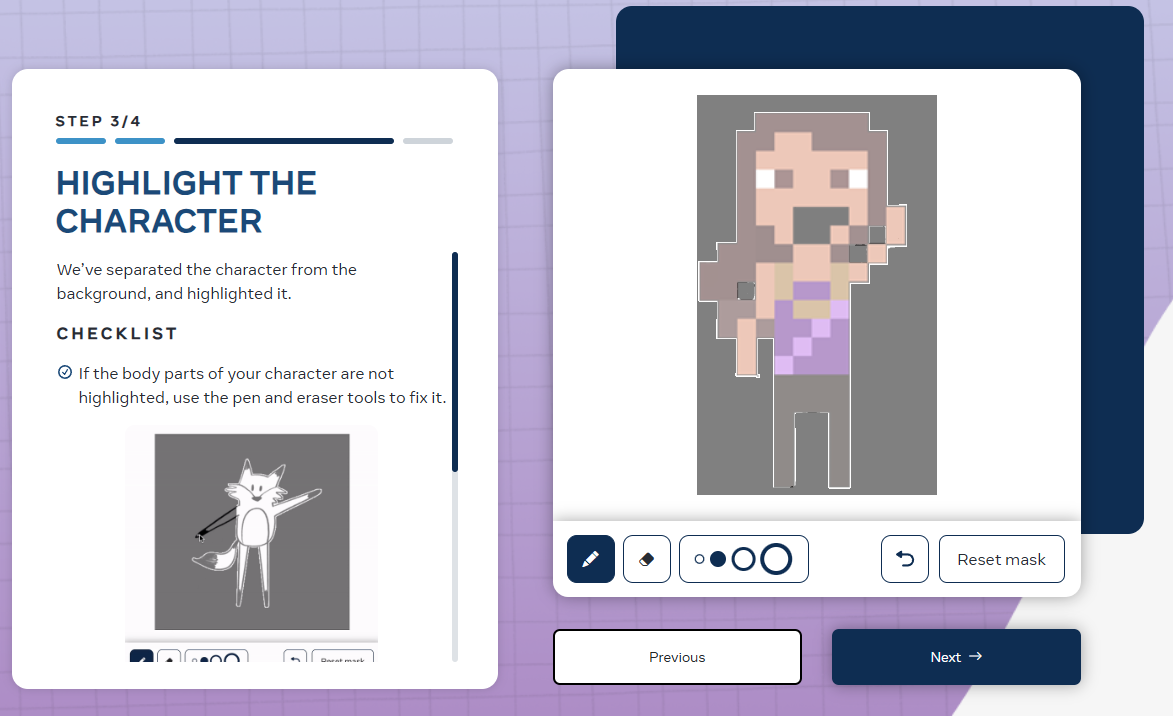
\includegraphics[width=1\linewidth]{figs/sketchLab/tela4.PNG}
        \caption{\small Destacar personagem manual.}
        \label{fig:sketch1d}
    \end{subfigure}
    \begin{subfigure}{0.45\linewidth}
        \centering
        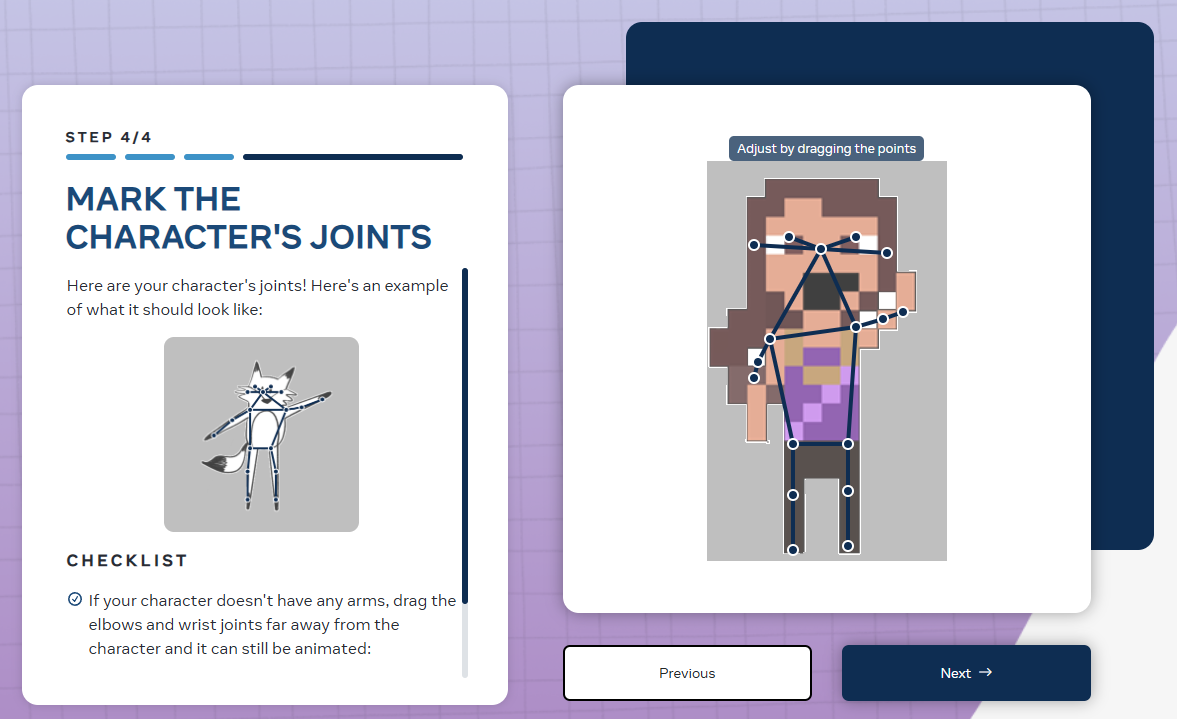
\includegraphics[width=1\linewidth]{figs/sketchLab/tela5.PNG}
        \caption{\small Marcar as articulações do personagem automático.}
        \label{fig:sketch1e}
    \end{subfigure}
    \begin{subfigure}{0.45\linewidth}
        \centering
        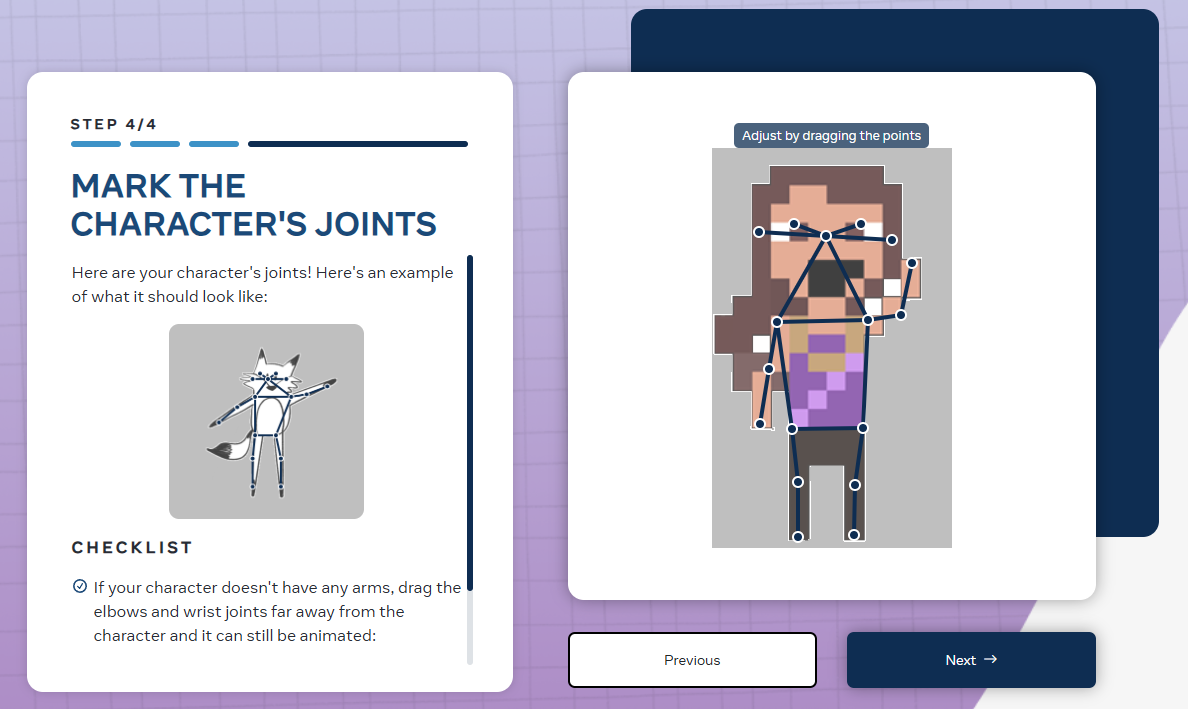
\includegraphics[width=1\linewidth]{figs/sketchLab/tela6.PNG}
        \caption{\small Marcar as articulações do personagem manual.}
        \label{fig:sketch1f}
    \end{subfigure}

    \legend{\small Fonte: Elaborada pela autora.}
\end{figure}

\begin{figure}[htbp]
    \centering
    \caption{\small Processo da utilização 2 do Animated Drawnings}
    \label{fig:sketch2}
    \begin{subfigure}{0.6\linewidth}
        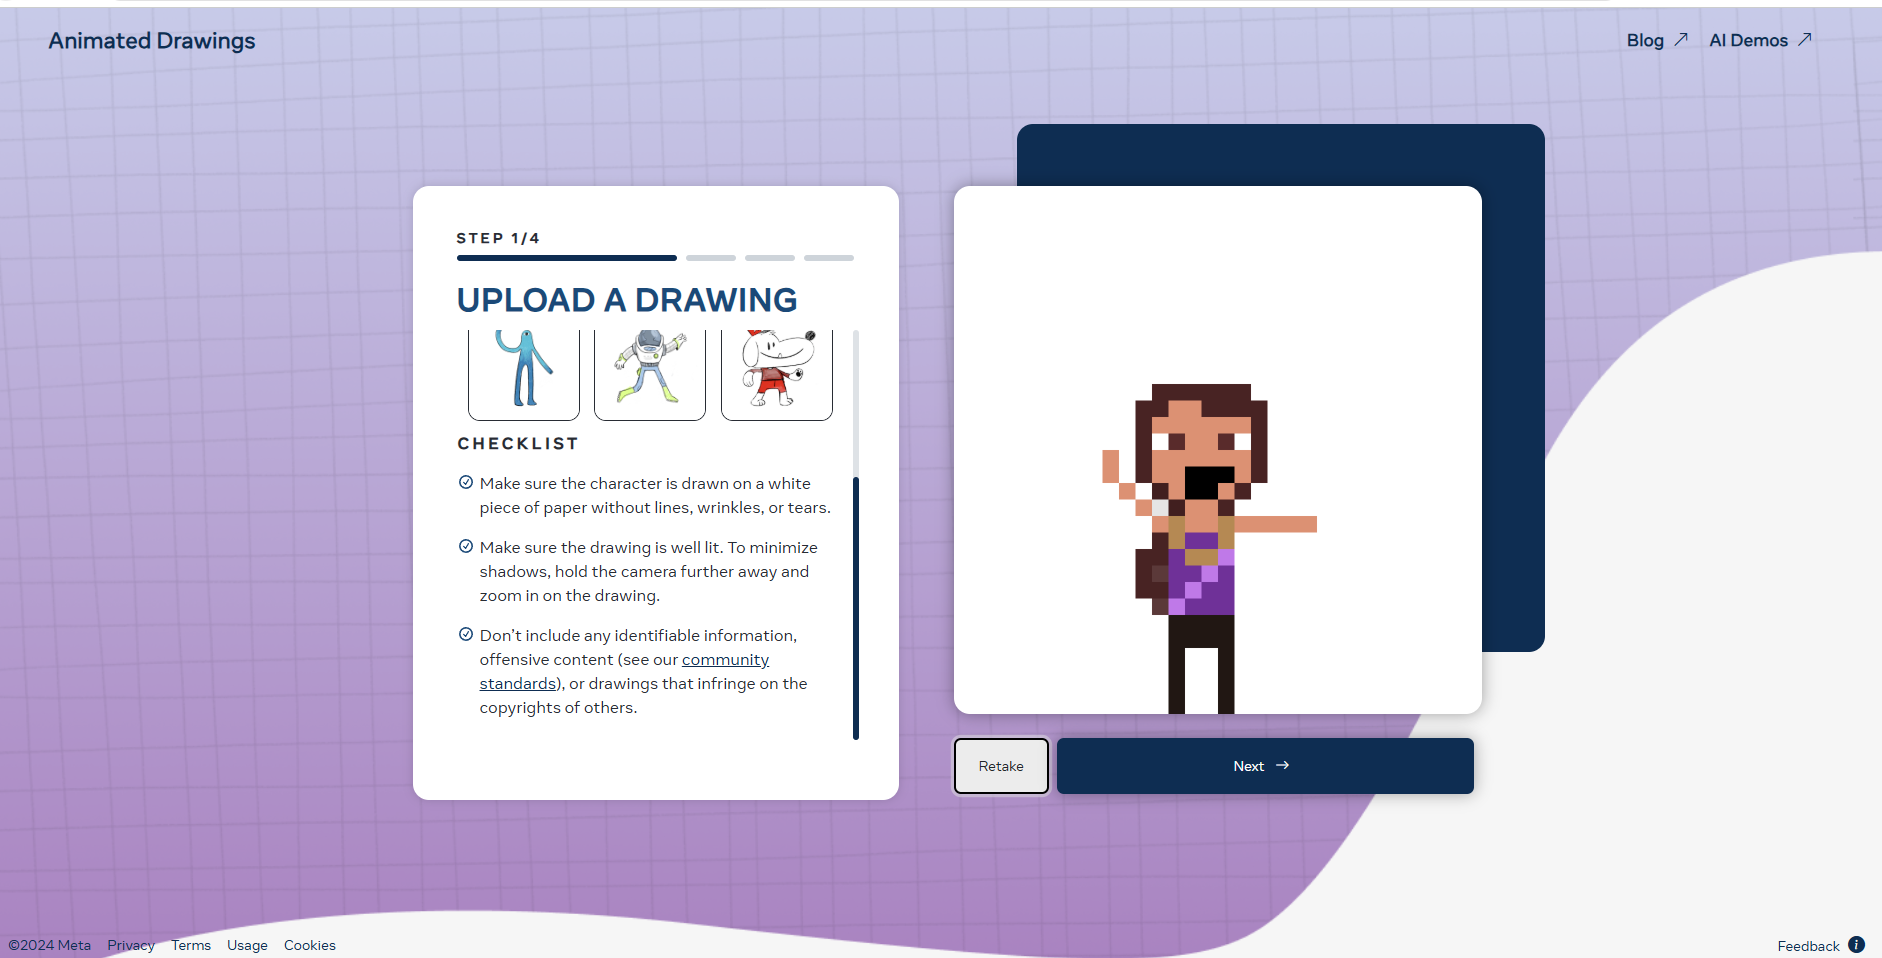
\includegraphics[width=1\linewidth]{figs/sketchLab/2tela1.PNG}
        \caption{\small Desenho enviado.}
        \label{fig:sketch2a}
    \end{subfigure}
    \begin{subfigure}{0.45\linewidth}
        \centering
        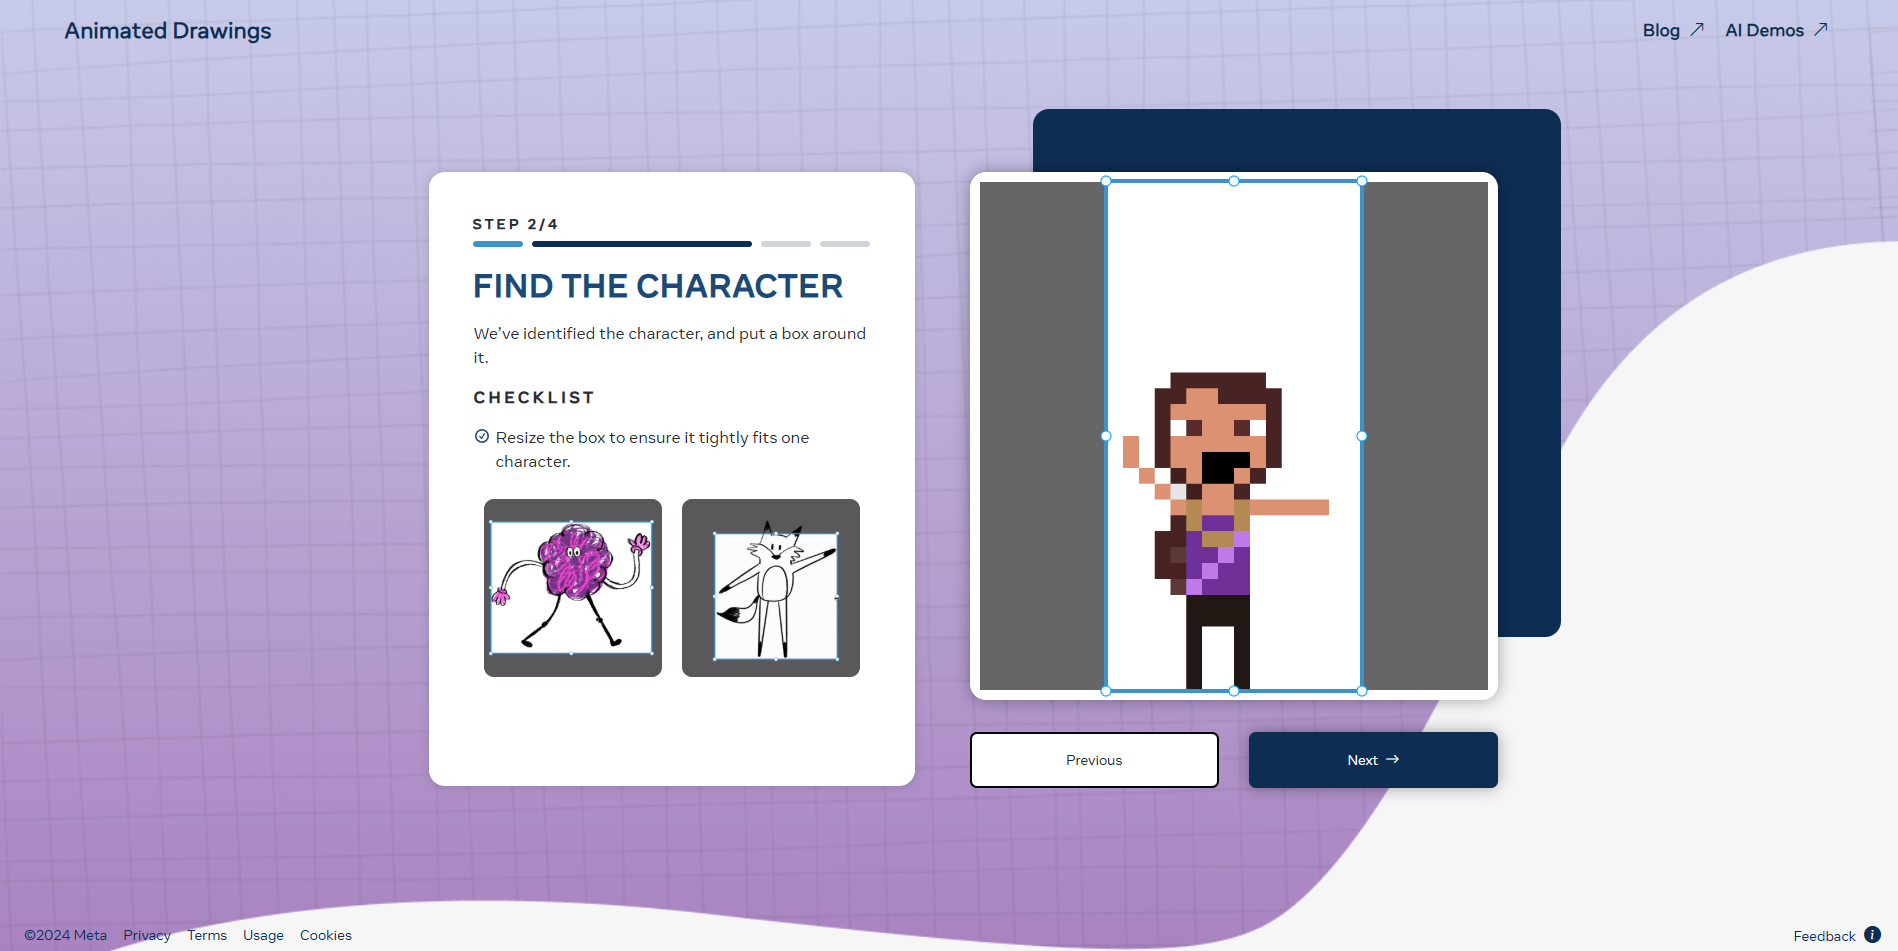
\includegraphics[width=1\linewidth]{figs/sketchLab/2tela2.PNG}
        \caption{\small Encontrar personagem automático.}
        \label{fig:sketch2b}
    \end{subfigure}
    \begin{subfigure}{0.45\linewidth}
        \centering
        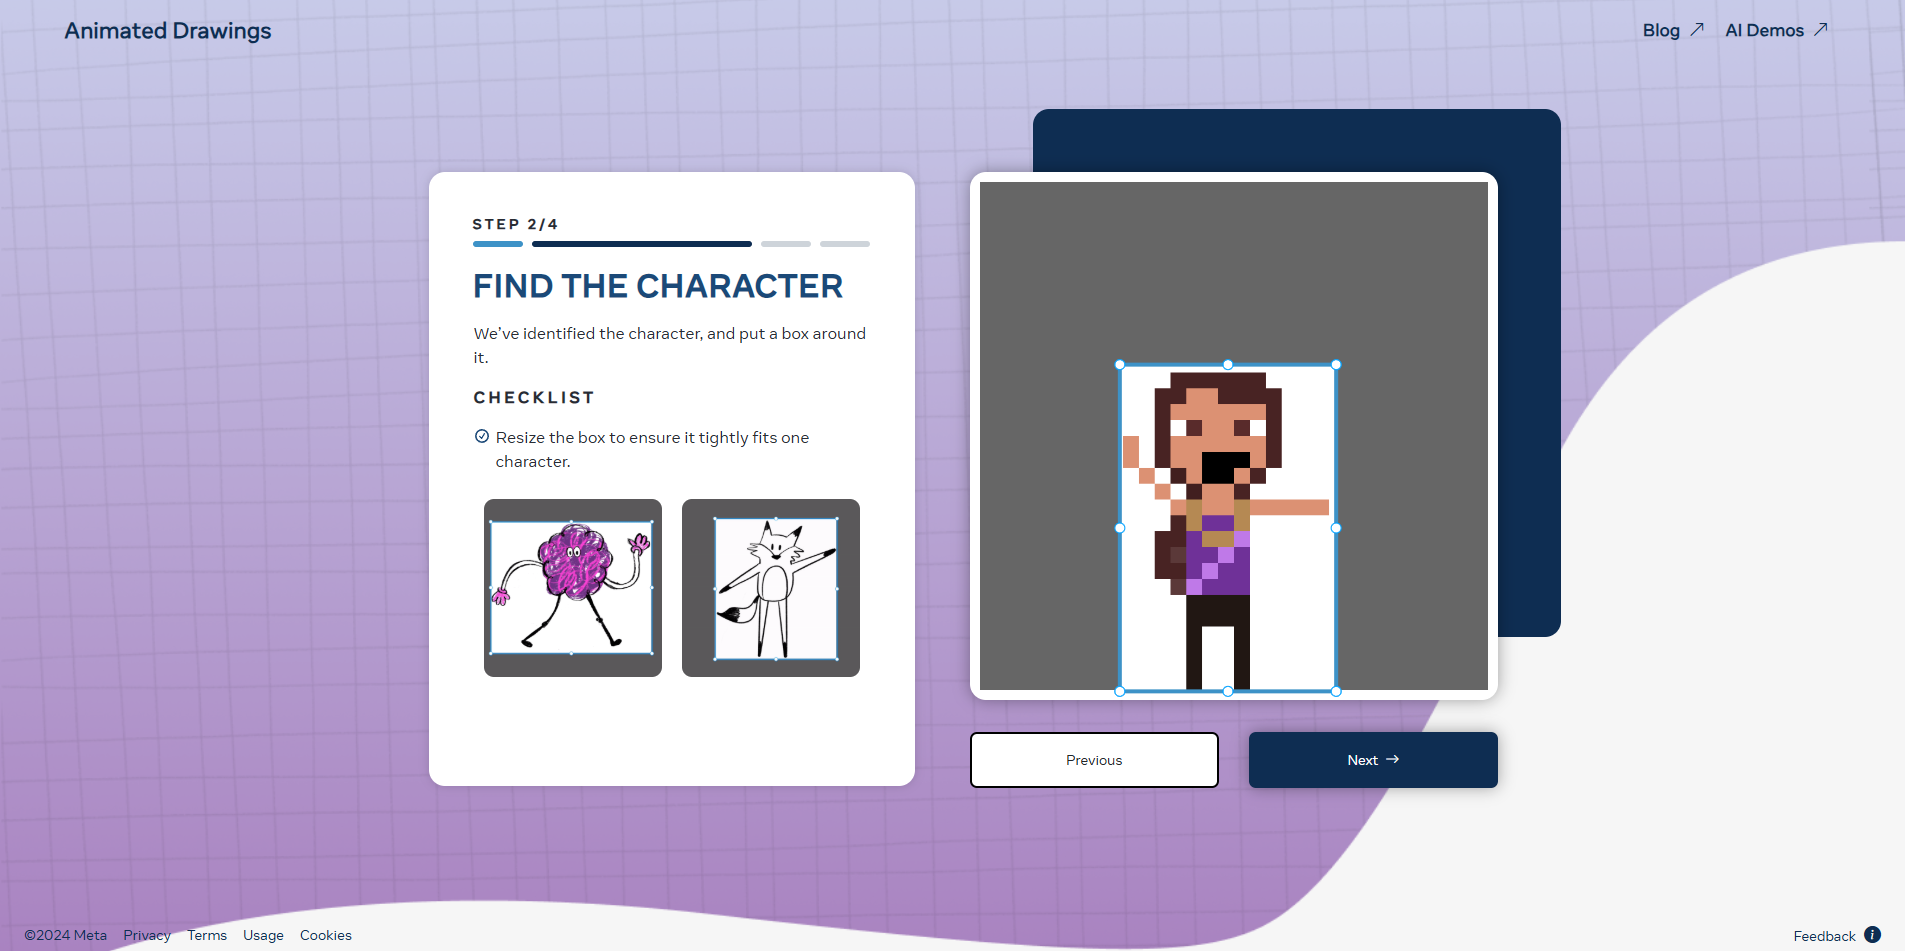
\includegraphics[width=1\linewidth]{figs/sketchLab/2tela3.PNG}
        \caption{\small Encontrar personagem manual.}
        \label{fig:sketch2c}
    \end{subfigure}
    \begin{subfigure}{0.45\linewidth}
        \centering
        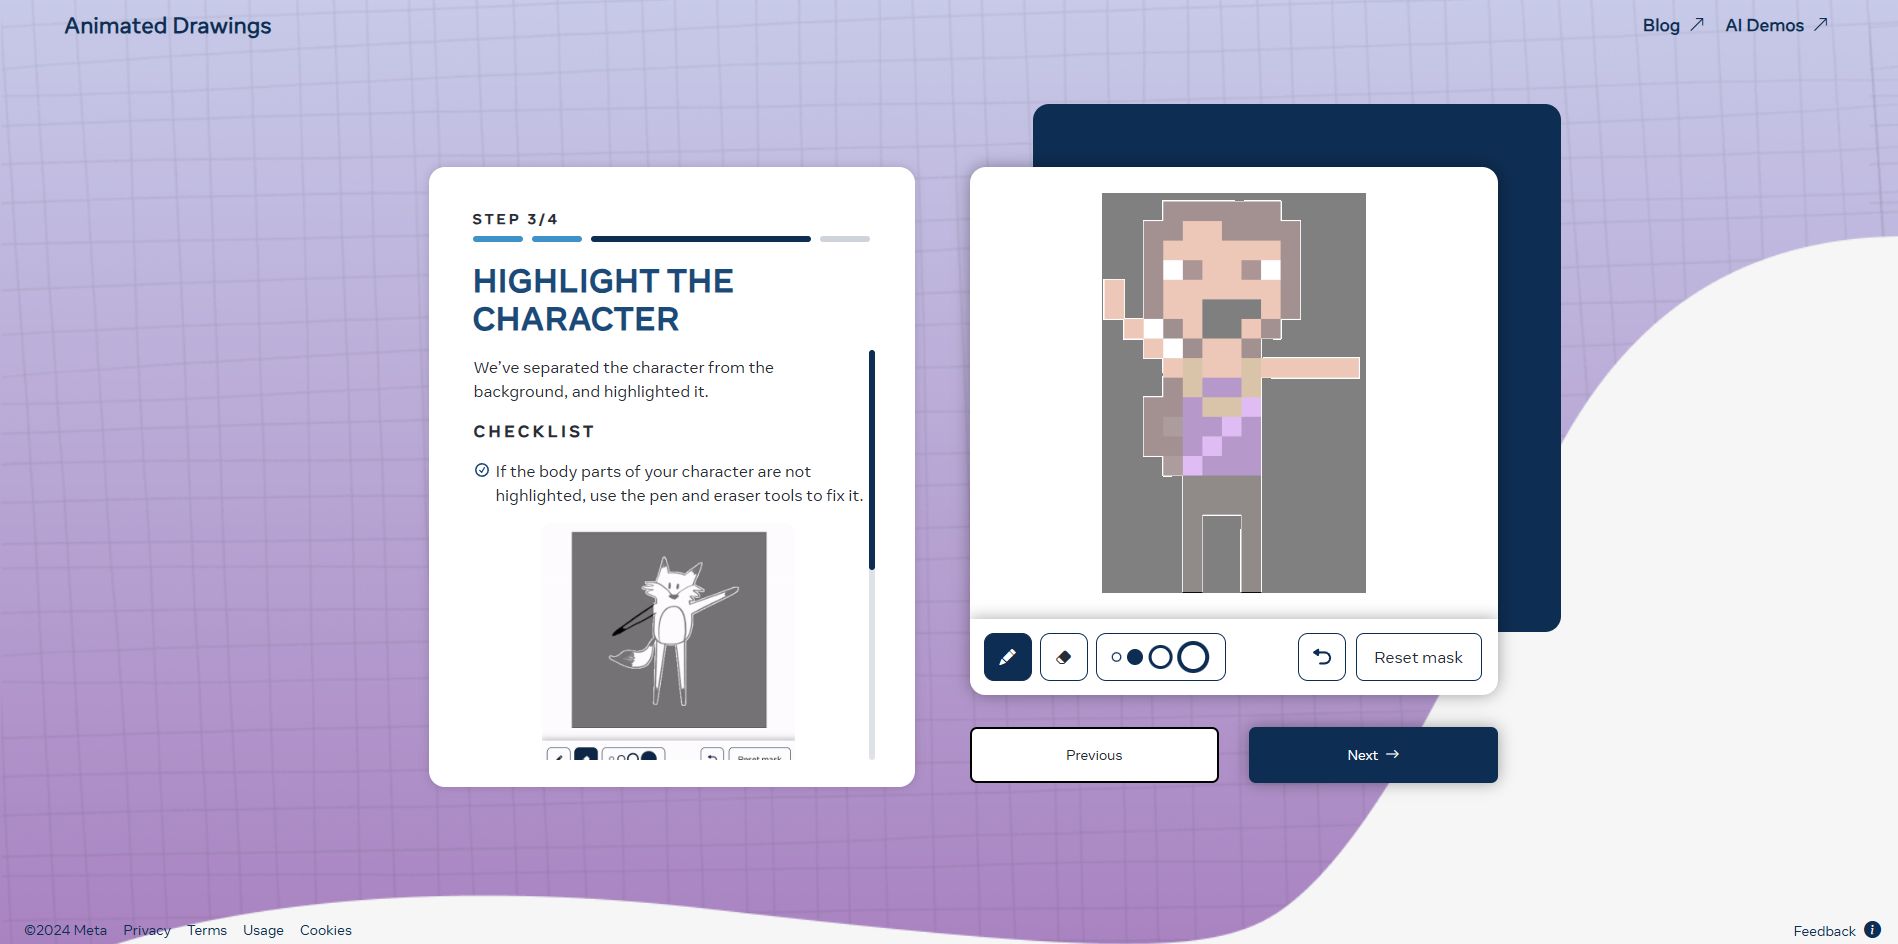
\includegraphics[width=1\linewidth]{figs/sketchLab/2tela4.PNG}
        \caption{\small Destacar personagem automático.}
        \label{fig:sketch2d}
    \end{subfigure}
    \begin{subfigure}{0.45\linewidth}
        \centering
        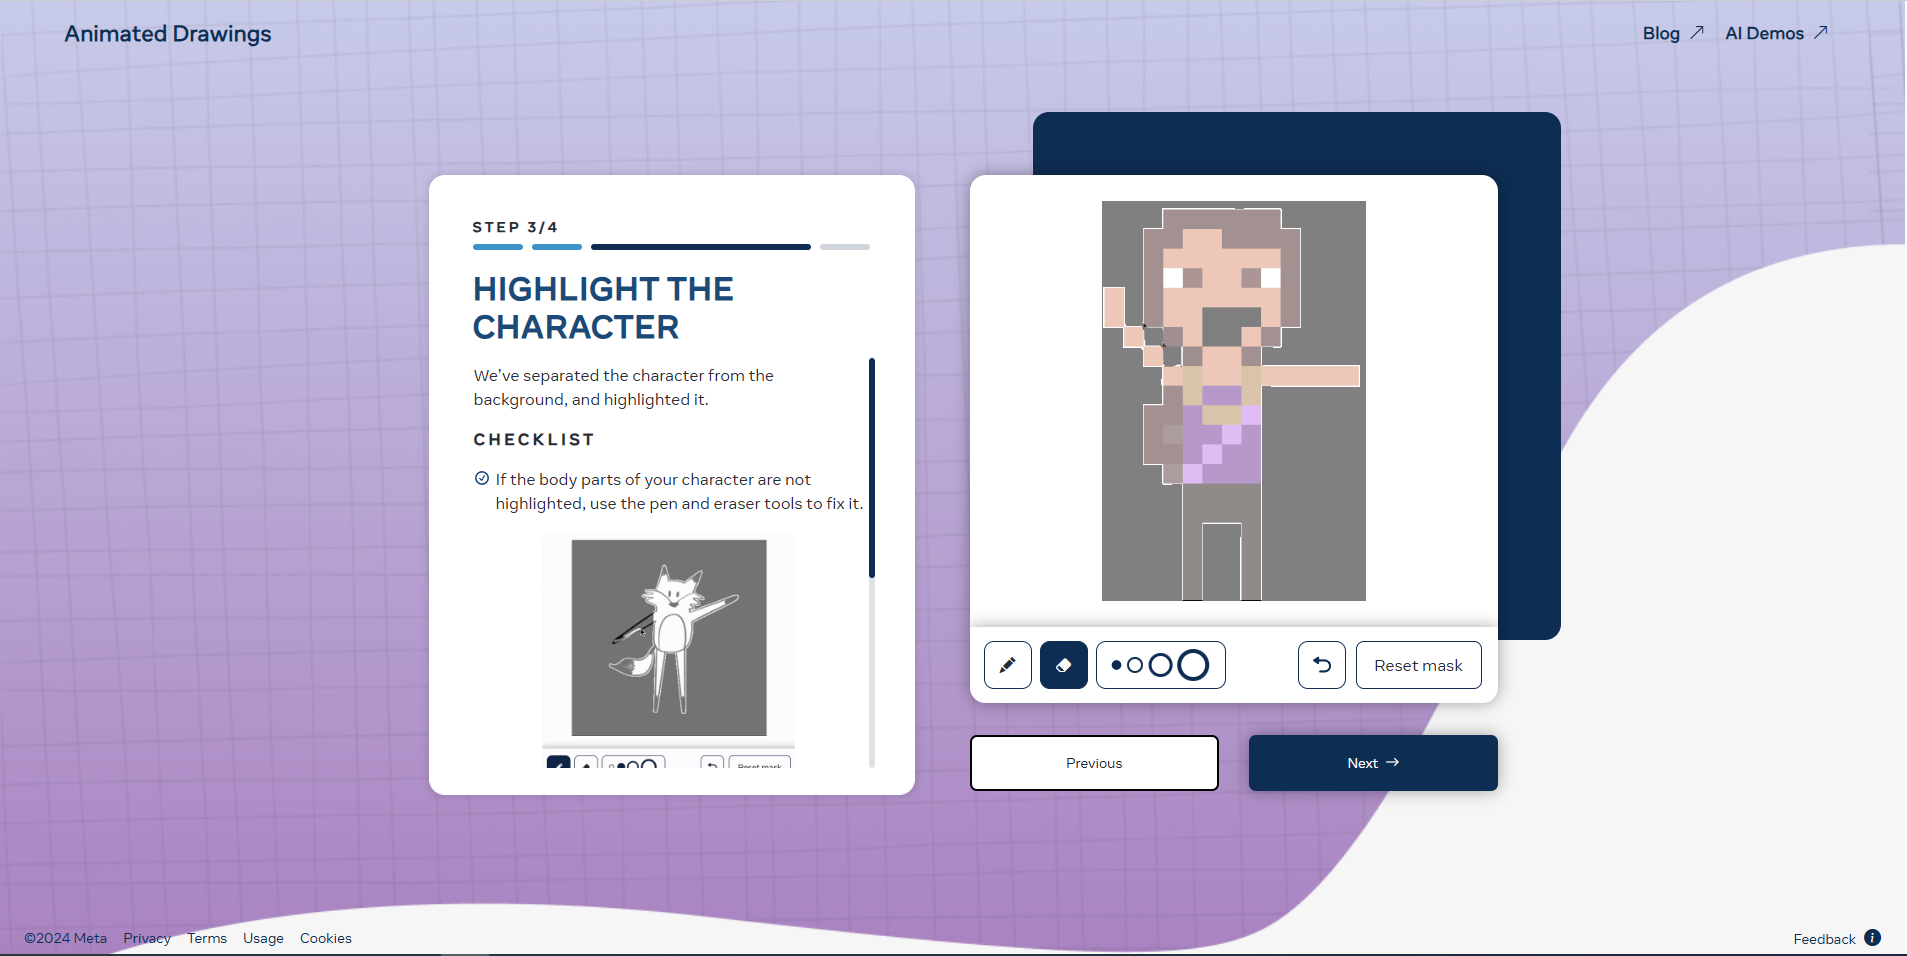
\includegraphics[width=1\linewidth]{figs/sketchLab/2tela5.PNG}
        \caption{\small Destacar personagem manual.}
        \label{fig:sketch2e}
    \end{subfigure}
    \begin{subfigure}{0.45\linewidth}
        \centering
        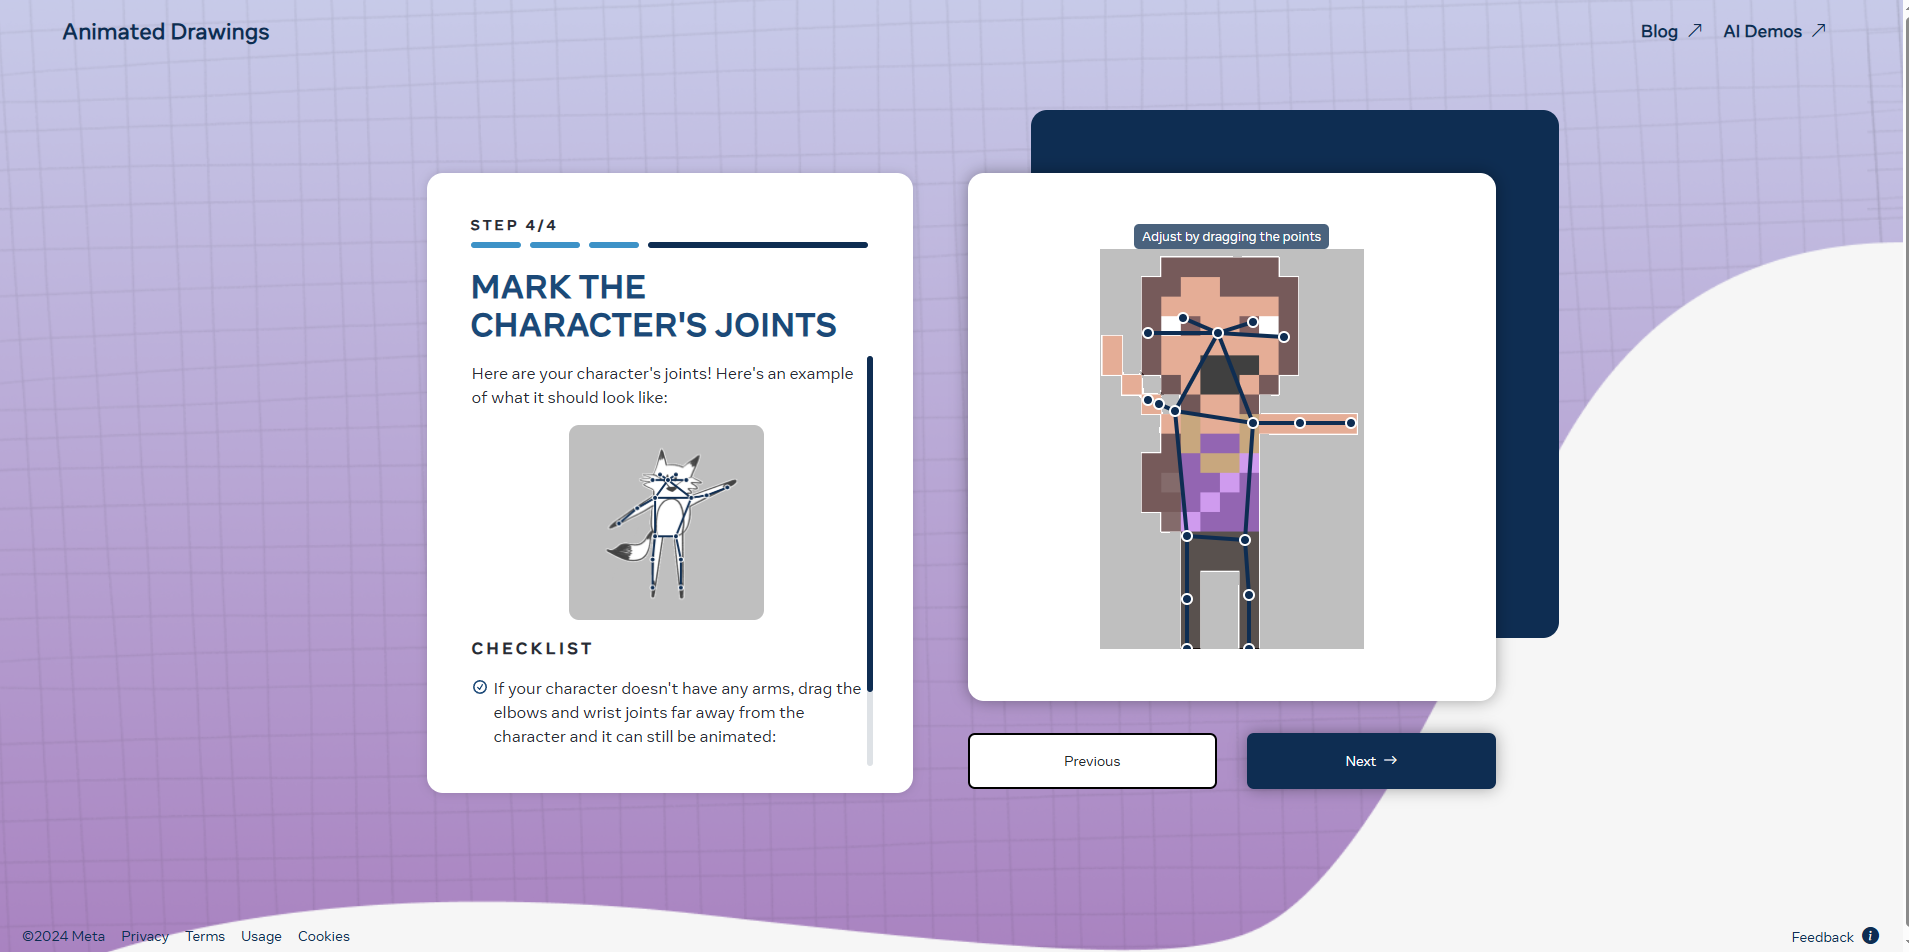
\includegraphics[width=1\linewidth]{figs/sketchLab/2tela6_2.PNG}
        \caption{\small Marcar as articulações do personagem automático.}
        \label{fig:sketch2f}
    \end{subfigure}
    \begin{subfigure}{0.45\linewidth}
        \centering
        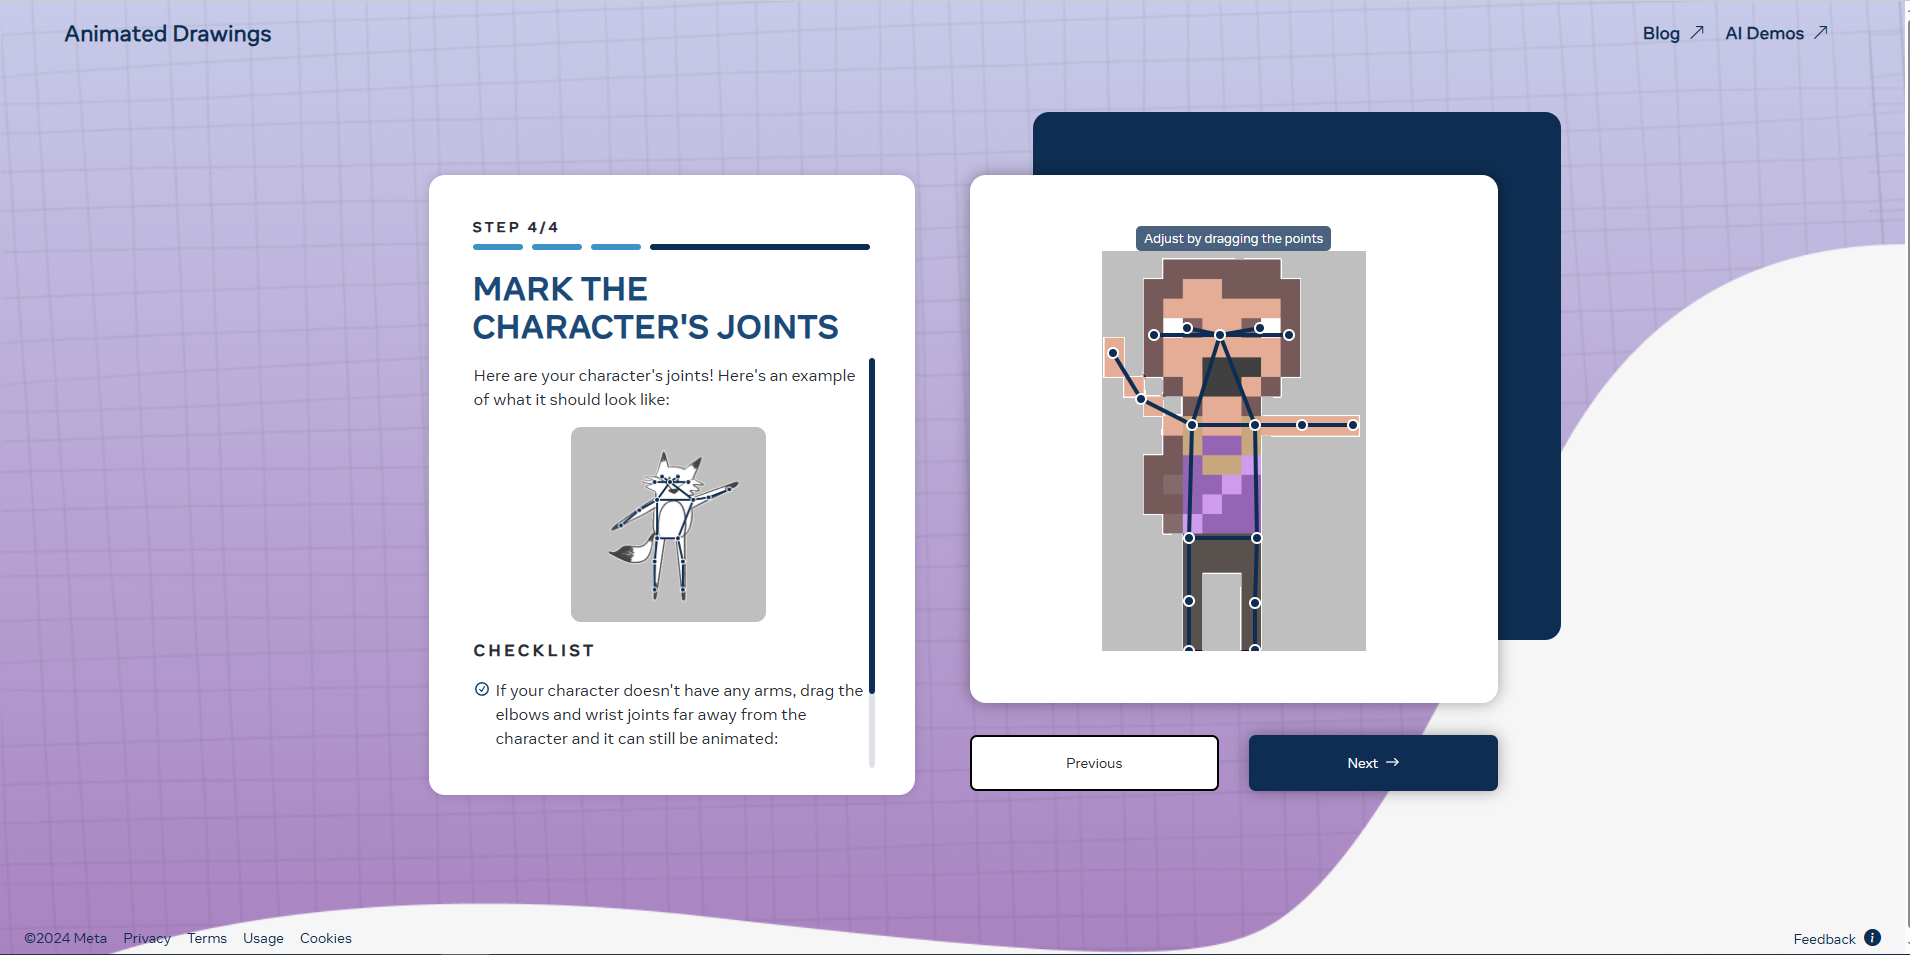
\includegraphics[width=1\linewidth]{figs/sketchLab/2tela7.PNG}
        \caption{\small Marcar as articulações do personagem manual.}
        \label{fig:sketch2g}
    \end{subfigure}

    \legend{\small Fonte: Elaborada pela autora.}
\end{figure}

\begin{figure}[htbp]
    \centering
    \caption{\small Processo da utilização 3 do Animated Drawnings}
    \label{fig:sketch3}
    \begin{subfigure}{0.45\linewidth}
        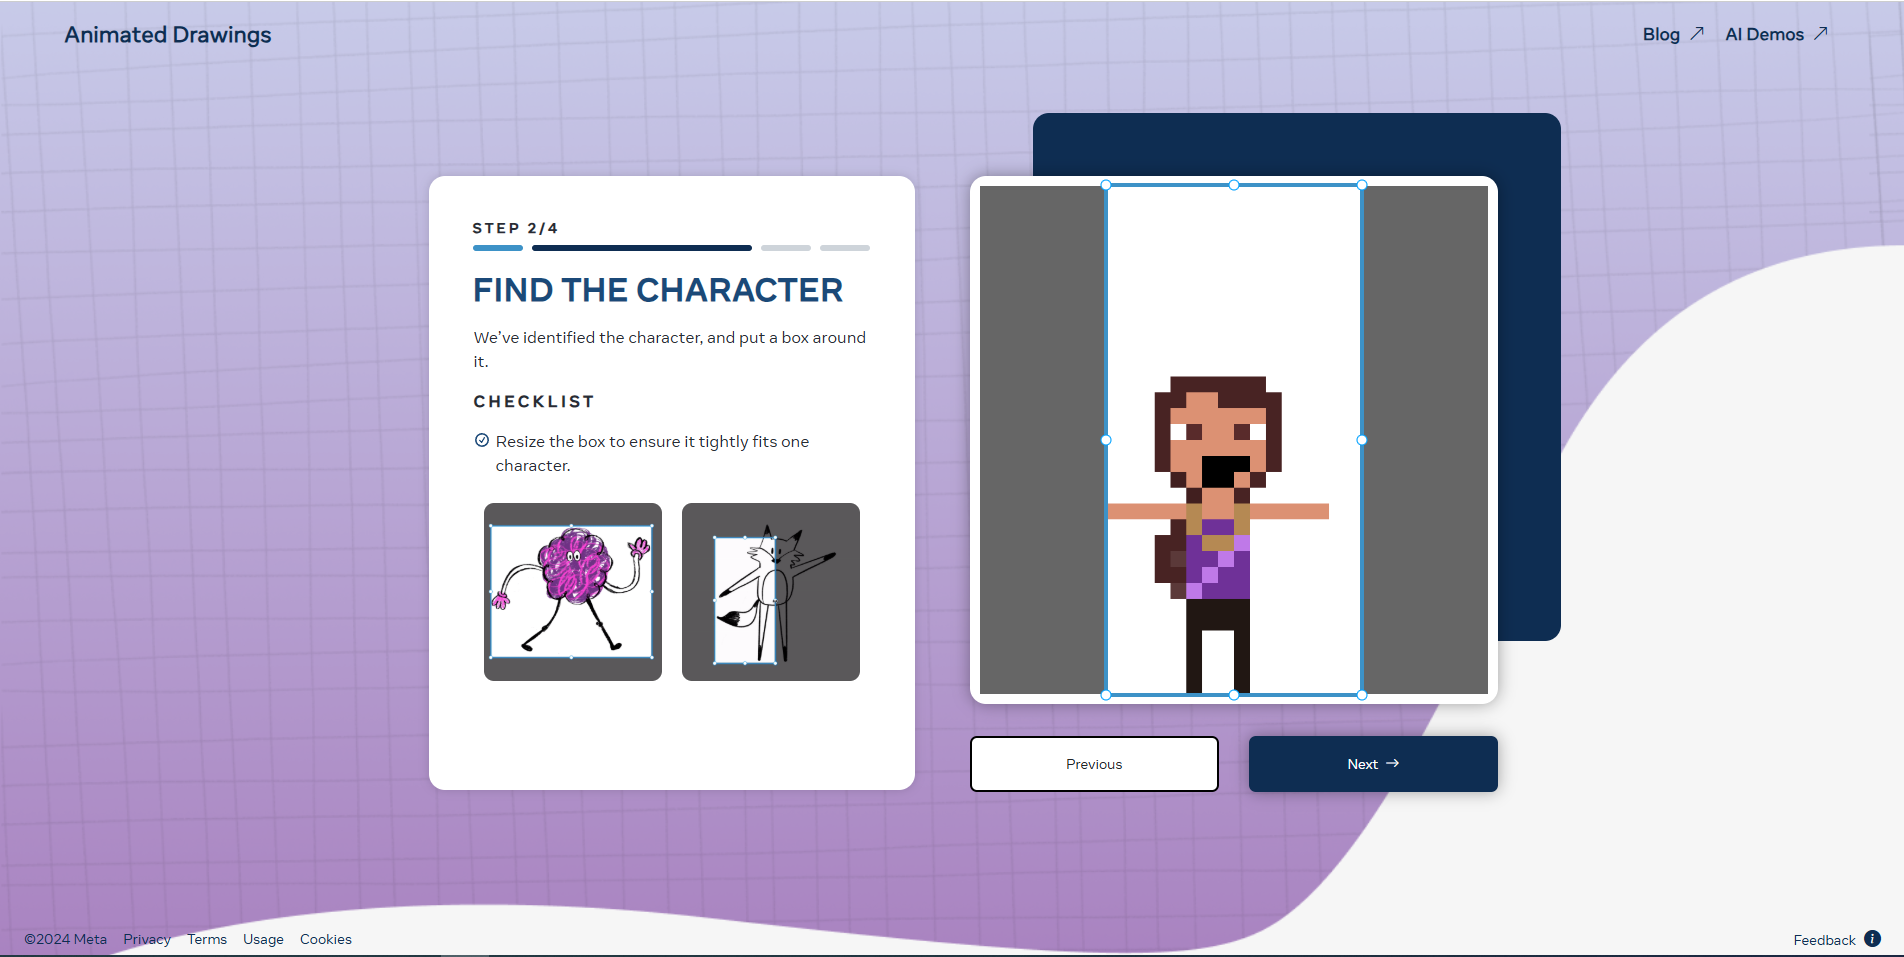
\includegraphics[width=1\linewidth]{figs/sketchLab/3tela1.PNG}
        \caption{\small Encontrar personagem automático.}
        \label{fig:sketch3a}
    \end{subfigure}
    \begin{subfigure}{0.45\linewidth}
        \centering
        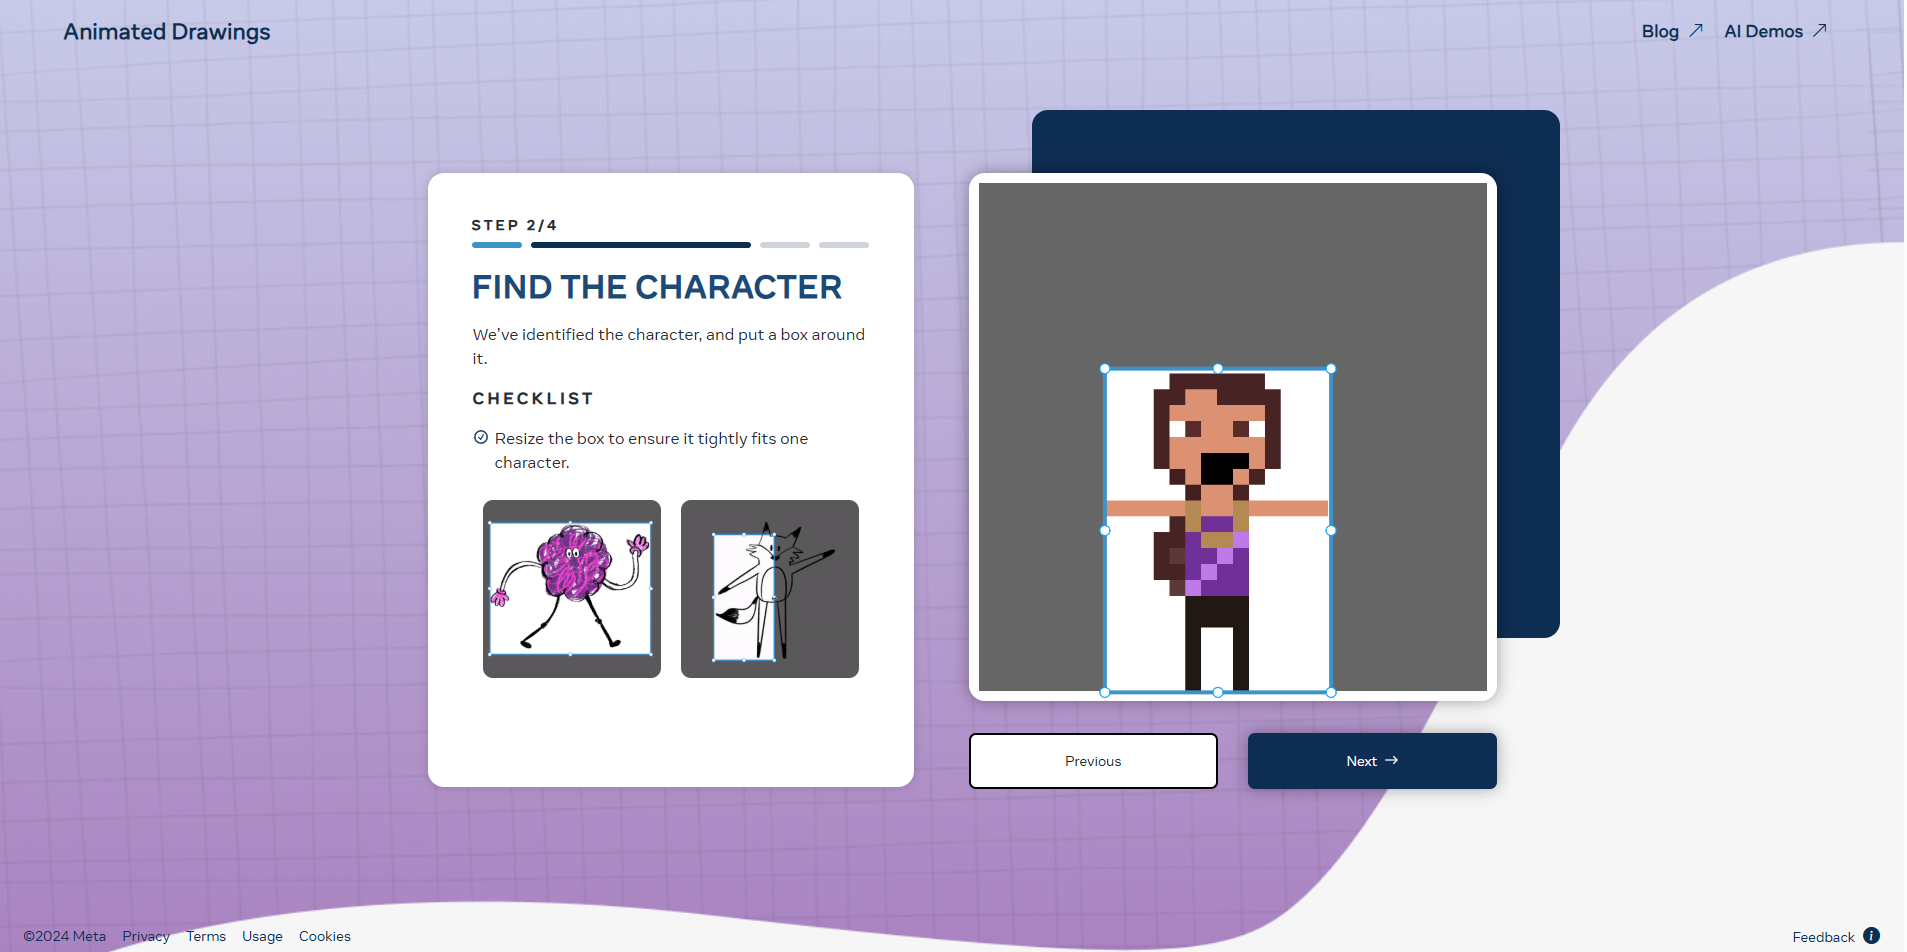
\includegraphics[width=1\linewidth]{figs/sketchLab/3tela2.PNG}
        \caption{\small Encontrar personagem manual.}
        \label{fig:sketch3b}
    \end{subfigure}
    \begin{subfigure}{0.6\linewidth}
        \centering
        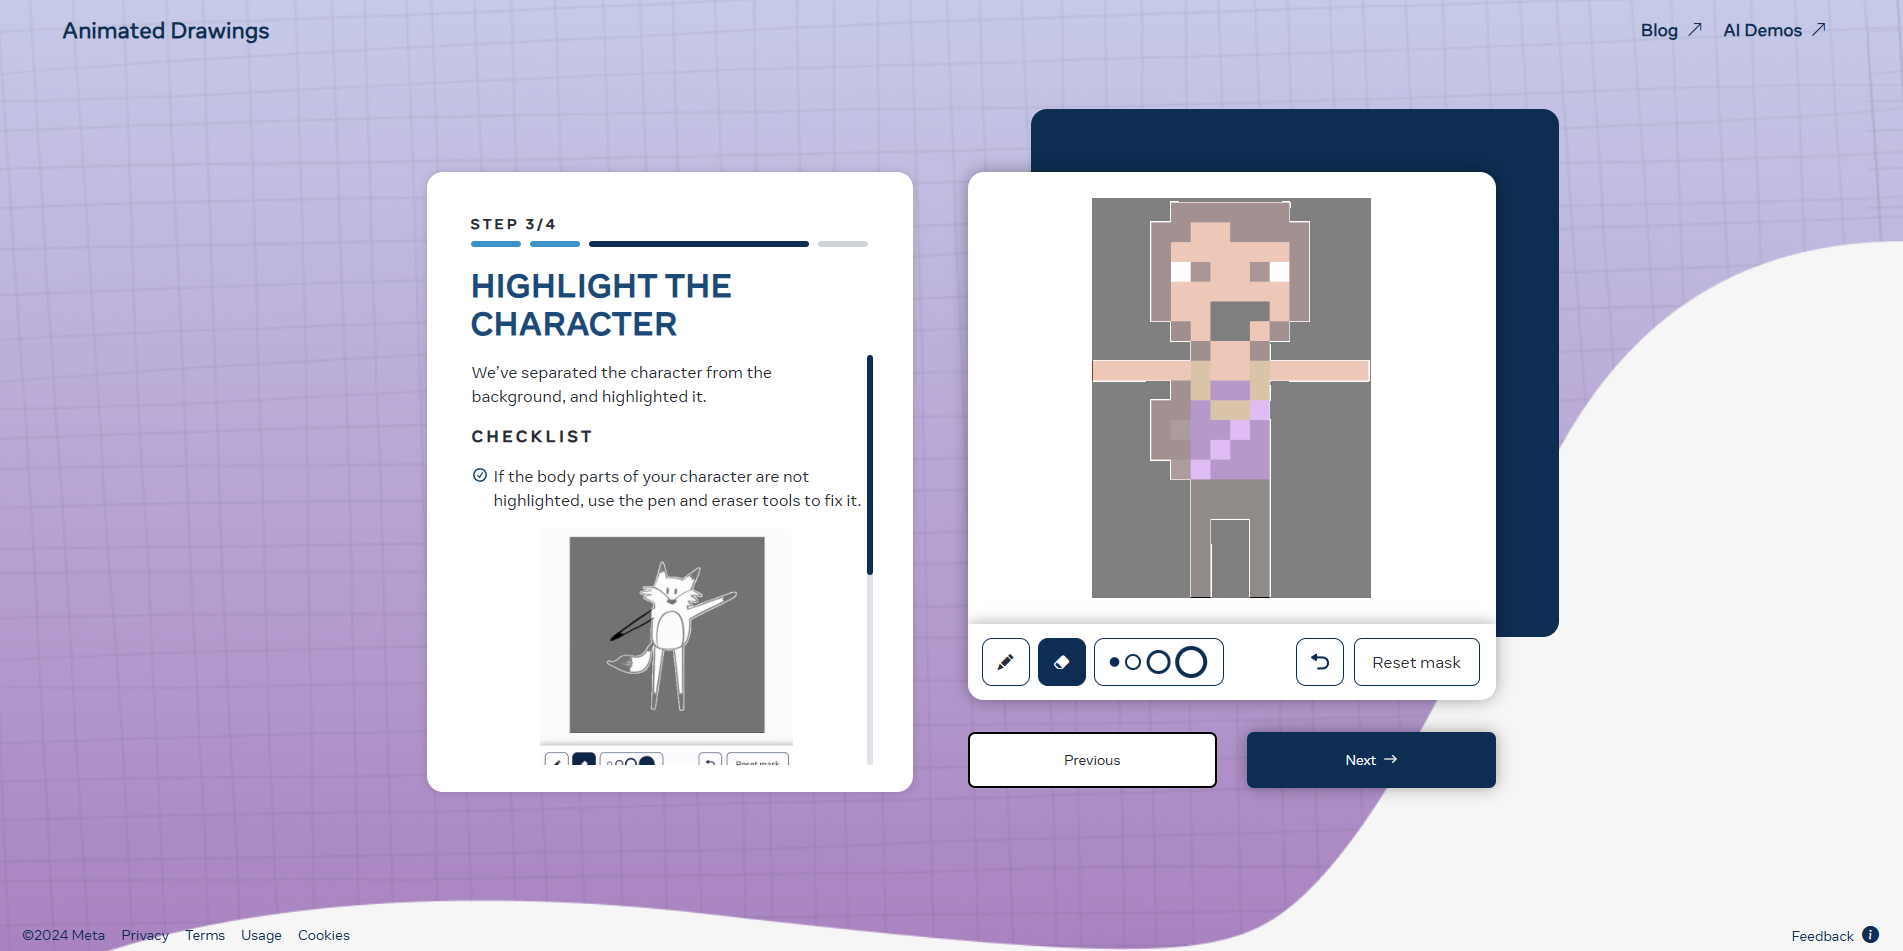
\includegraphics[width=1\linewidth]{figs/sketchLab/3tela3.PNG}
        \caption{\small Destacar personagem automático.}
        \label{fig:sketch3c}
    \end{subfigure}
    \begin{subfigure}{0.45\linewidth}
        \centering
        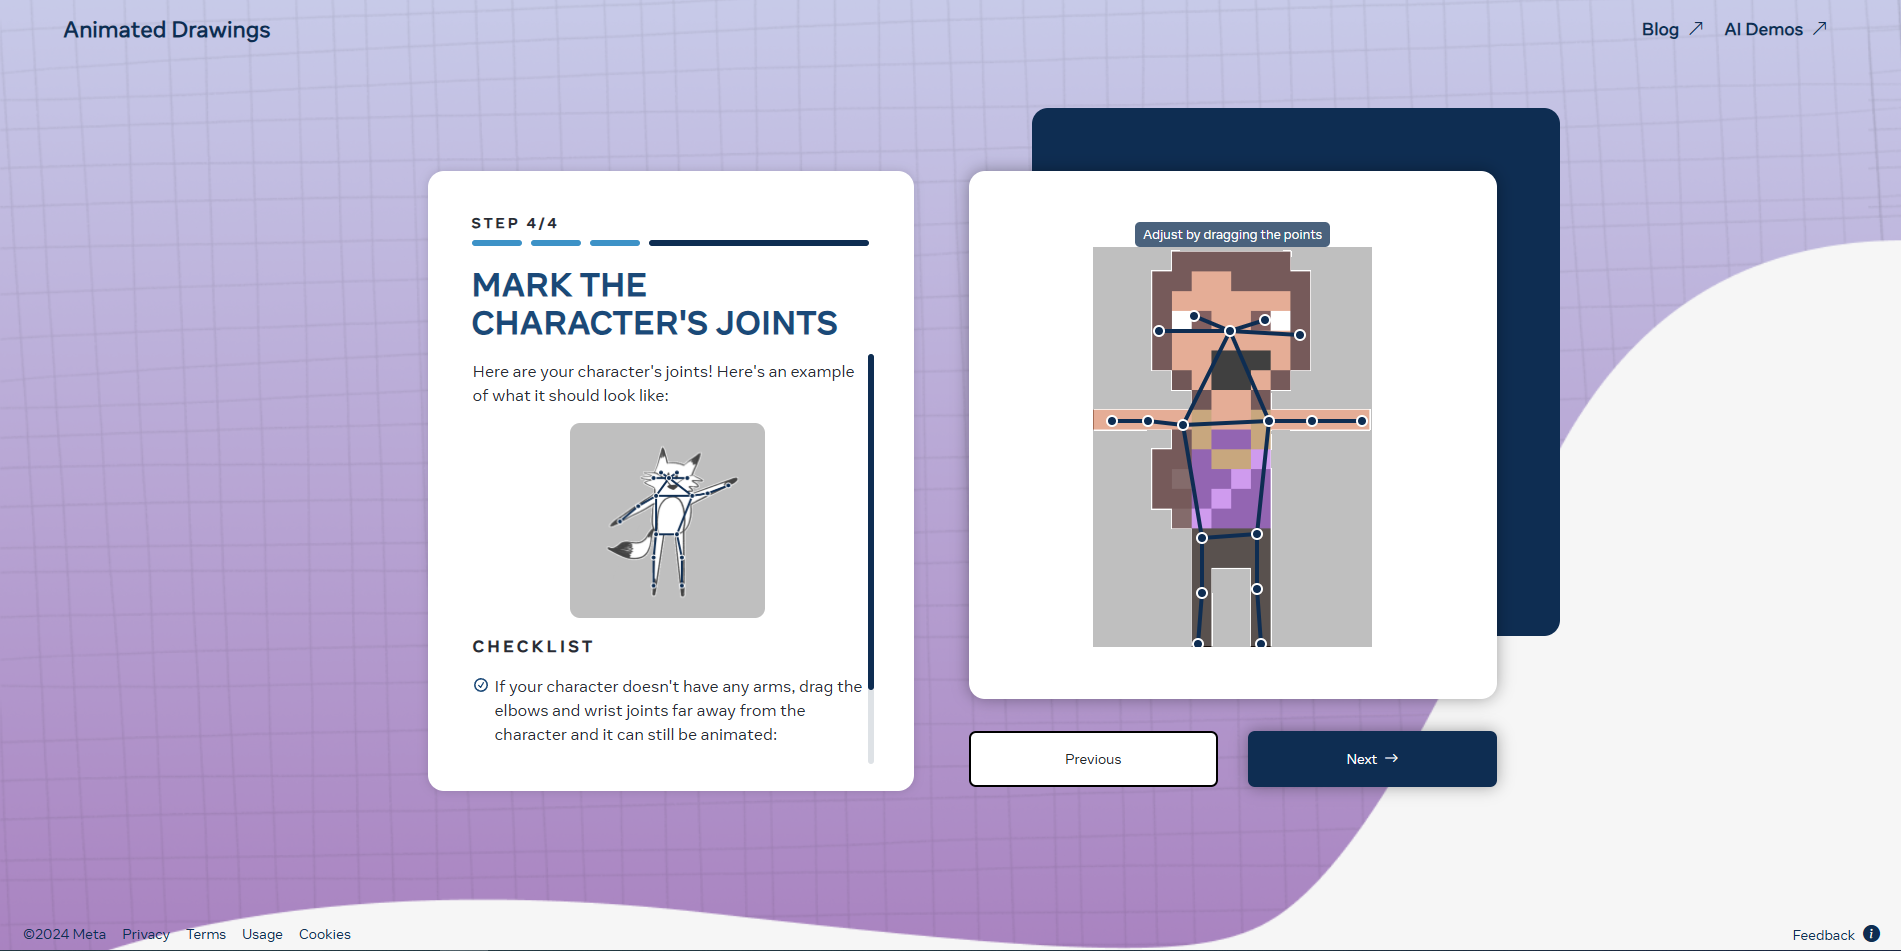
\includegraphics[width=1\linewidth]{figs/sketchLab/3tela4.PNG}
        \caption{\small Marcar as articulações do personagem automático.}
        \label{fig:sketch3d}
    \end{subfigure}
    \begin{subfigure}{0.45\linewidth}
        \centering
        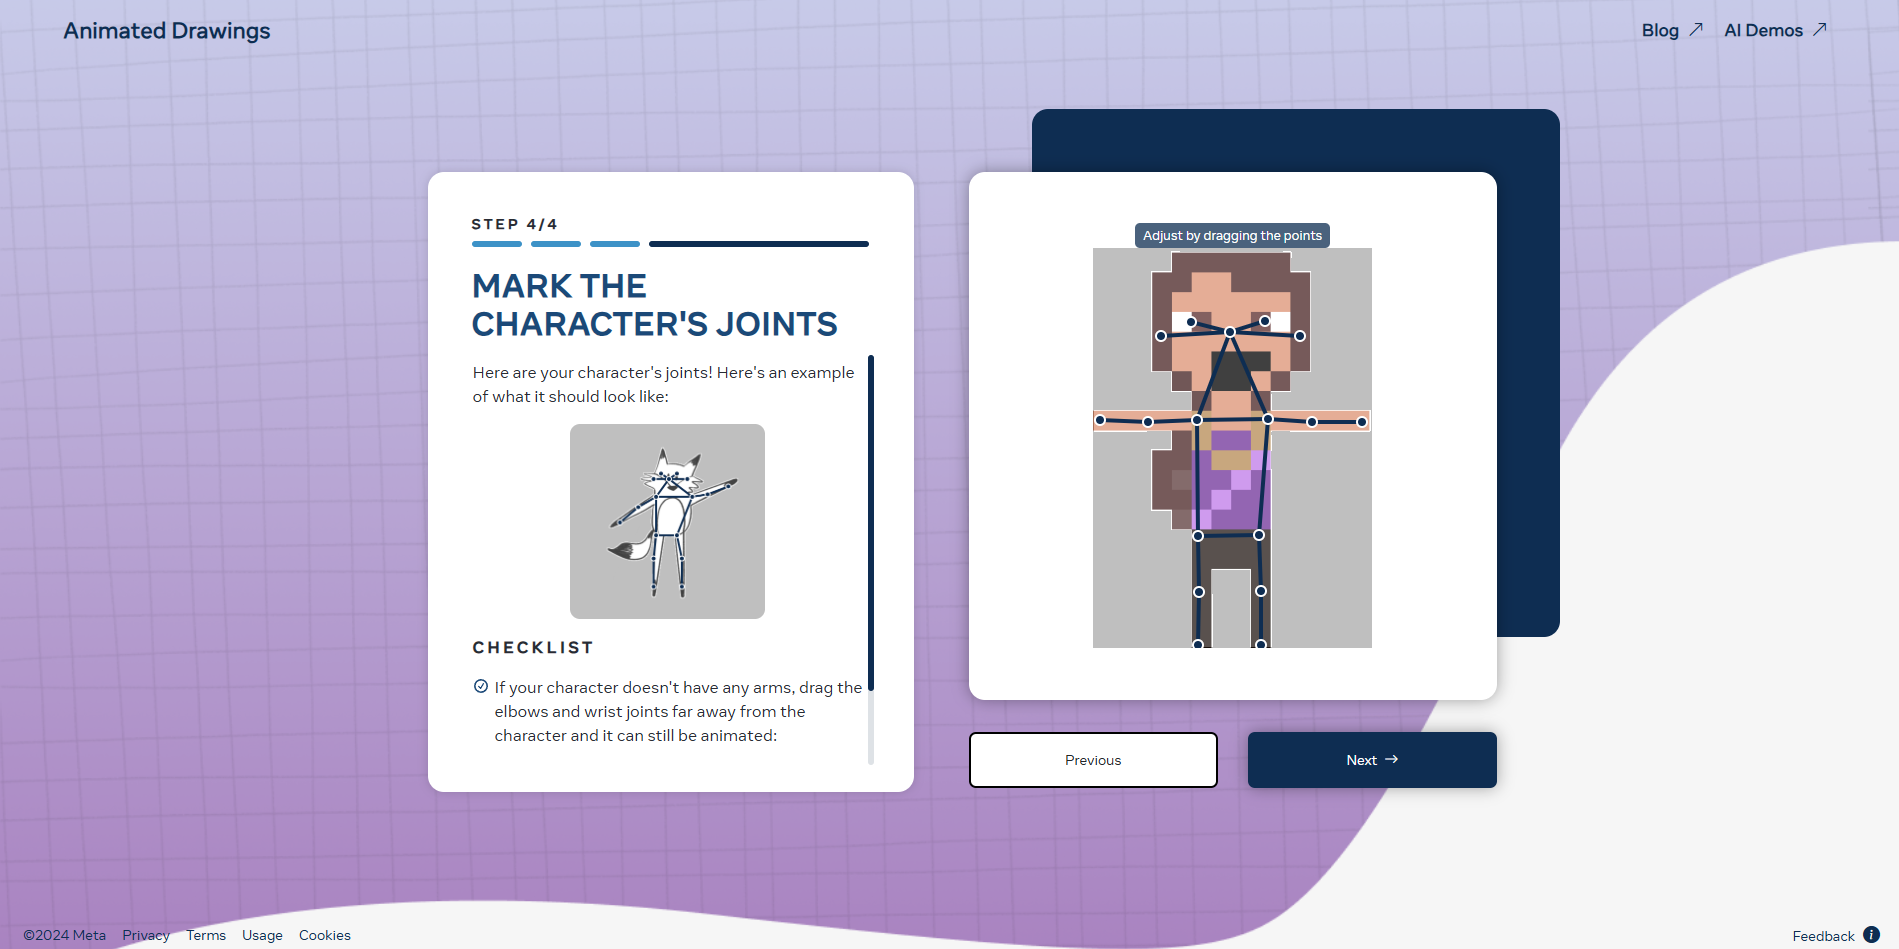
\includegraphics[width=1\linewidth]{figs/sketchLab/3tela6.PNG}
        \caption{\small  Marcar as articulações do personagem manual}
        \label{fig:sketch3e}
    \end{subfigure}
    \legend{\small Fonte: Elaborada pela autora.}
\end{figure}